% !TeX root = ../thuthesis-example.tex

\chapter{服务器端高性能 \emph{insertRecords} 写入机制设计与实现}
经过客户端的预处理与 RPC 层的数据传输,写入请求最终会到达服务器端。服务器端对写入请求进行预处理后,交由存储引擎负责处理写入请求,并将这些数据最终持久化到磁盘上,服务器端的设计与实现对写入性能有至关重要的影响。如 \ref{sec:chap3-sec3-1} 中的实验结果所示,现有 IoTDB 服务器端对写入请求的处理有较大的性能瓶颈,不能满足高并发写入请求的需求。因此,本章将介绍对 \emph{insertRecords} 写入请求所设计的服务器端高性能写入机制。


\section{服务器端 \emph{insertRecords} 写入流程总览}
\ref{sec:chap3-sec2} 节介绍了 IoTDB 服务器端对 \emph{insertRecords} 写入请求执行的总体流程,新的执行流程和原有流程大体相似,单针对之前实验中发现的瓶颈,本工作进行了重新设计以优化写入性能。

\begin{figure}
  \centering
  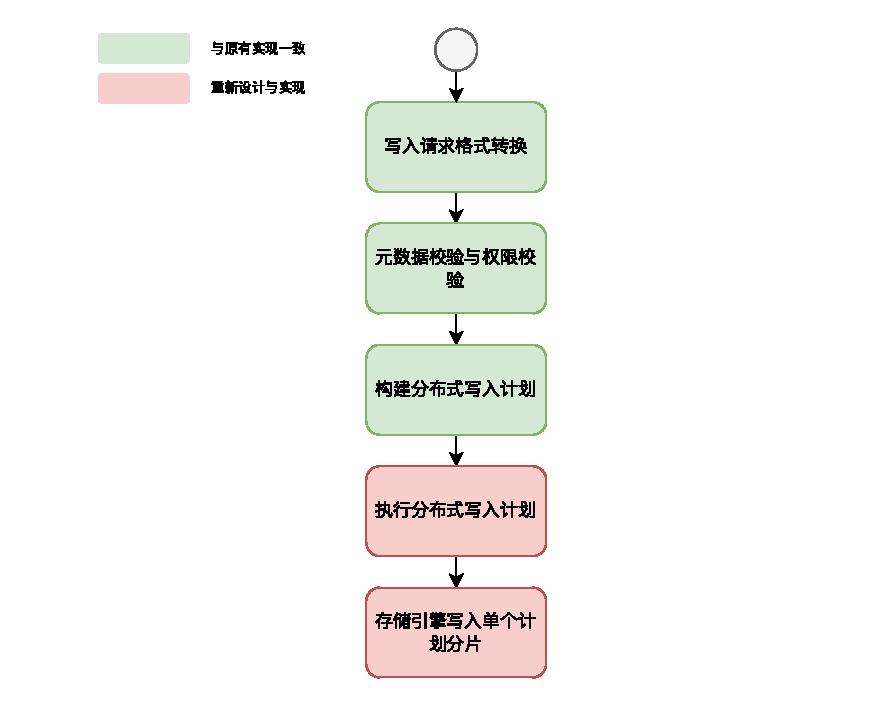
\includegraphics[width=0.9\linewidth]{new-storage-engine.pdf}
  \caption{服务器端 \emph{insertRecords} 写入流程}
  \label{fig:iotdb-insertRecords-flow}
\end{figure}

图 \ref{fig:iotdb-insertRecords-flow} 展示了 \emph{insertRecords} 写入请求到达 IoTDB 服务器端以后的总体执行流程,其中绿色部分代表这些流程与 IoTDB 原有设计基本保持一致,因为它们并不是写入的瓶颈所在;红色部分代表了在原有实现中存在的性能瓶颈,本工作对这些部分进行了重新设计与实现以提高写入性能。


在执行分布式写入计划时,一个写入请求会被分为多个写入计划分片(称为 FragmentInstance,FI),每个分片都是写入到一个 DataRegion 中的计划。根据 DataRegion 的分布,可以将其分为本地 DataRegion 和远程 DataRegion,本地 DataRegion 是指存储引擎所在的节点上的 DataRegion,远程 DataRegion 是指存储引擎所在节点以外的 DataRegion。为了充分利用多核 CPU 的计算能力,本工作将写入本地和写入远程 DataRegion 的过程都设计为了多线程并行执行,以提高写入性能。

在存储引擎写入单个计划分片时,不仅需要将数据记录到内存表中,还需要执行记录写前日志、更新监控信息、维护内存索引等操作。这些操作大部分都不是核心的写入操作,但是却会对写入性能产生较大的影响。因此,本工作通过批量化的形式,将这些操作的代价分摊到多行写入记录上,以减少这些操作对写入性能的影响。例如,原本每写入一行记录就需要记录一次写前日志、更新一次监控信息、维护一次内存索引,现在可以将这些操作批量化,每写入一批记录才执行一次这些操作,这样平均到每一条记录上的代价就大大减小了。最后,为了改善前文提到的使用 \emph{insertRecords} 接口进行写入时写前日志过多的问题,本工作对写前日志进行了压缩,减少了写前日志对磁盘的写入量,提高了写入性能。下面将详细介绍这些优化措施的设计与实现。

\section{多线程并行写入设计与实现}
\subsection{多线程并行写入设计}
图 \ref{fig:fi-parallel-write} 展示了 FragmentInstance 多线程并行写入的总体架构。多线程并行写入的设计分为写入本地 DataRegion 和写入远程 DataRegion 两部分,下面将分别介绍这两部分的设计。

\begin{figure}
  \centering
  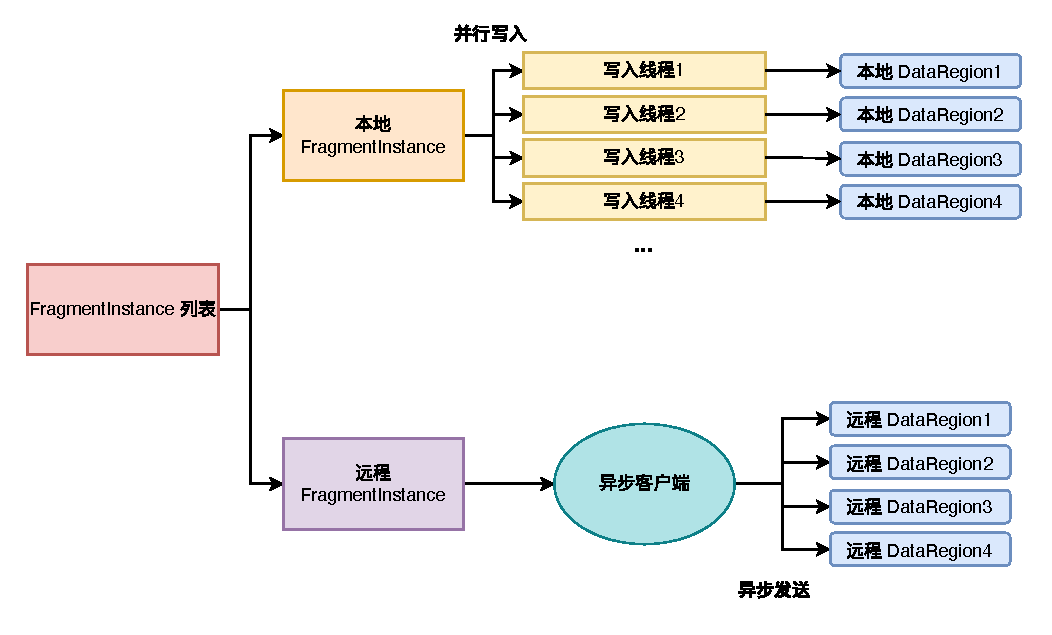
\includegraphics[width=\linewidth]{FragmentInstance写入.pdf}
  \caption{多线程并行写入设计}
  \label{fig:fi-parallel-write}
\end{figure}

在一般的系统中,对一项任务的并行执行通常会构建一个线程池负责此工作,以减少线程创建与销毁的开销,在本工作的设计中遵循了这一种范式。因此,想要实现多线程并行写入,我们首先要确定线程池的大小。如果线程池中的线程数过少,那么无法充分利用多核 CPU 的计算能力,从而无法提高写入性能;如果线程池中的线程数过多,那么会增加线程创建与销毁的开销,反而会降低写入性能。根据线程数与 DataRegion 的个数的比例,可以分为多个线程写一个 DataRegion、一个线程写一个 DataRegion 和一个线程写多个 DataRegion 三种情况。在目前 IoTDB 的设计与实现中,每个 DataRegion 都有一个锁,用于保证对 DataRegion 的读写操作是线程安全的。此外,一个 DataRegion 也对应了一个共识组,共识层为了保证数据的一致性,也持有一个锁。在这样的设计下,针对一个 DataRegion 的写入是串行的,即一次只能有一个线程写入一个 DataRegion。

综合以上因素,本工作选择了一个线程写一个本地 DataRegion 的设计,即每个 DataRegion 都有一个专门的线程负责处理这个 DataRegion 的写入任务。为了处理多个写入请求,每个 DataRegion 的线程都会维护一个写入队列,用于存放待写入的数据。不同写入请求对同一个 DataRegion 的写入任务会被放入同一个队列中,该 DataRegion 对应的写入线程会不断从写入队列中取出任务进行处理。为了避免过多任务堆积,任务队列的大小是有限的,超过了队列的大小后,新的写入请求会被拒绝,并向客户端返回写入失败的信息。写入请求向写入队列提交写入任务后,会获得一个 Future 对象,用于知晓写入任务的执行结果。写入任务执行完成后,Future 对象会被设置为完成状态,并且可以通过 Future 对象获取写入任务的执行结果。

对远程 DataRegion 的写入通过网络发送,在系统内缓存了一个全局的客户端池,它们负责将对远程 DataRegion 写入的 FragmentInstance 异步地发送到对应的节点上,并且返回一个 Future 对象,用于后续的处理。

当写入本地 DataRegion 和远程 DataRegion 的 FragmentInstance 都被异步地分发之后,主写入线程会拿到所有这些 FragmentInstance 对应的 Future 对象,并通过这些对象等待它们全部完成,随后将写入结果返回给客户端。

\subsection{多线程并行写入实现}
为了实现上述的设计,本工作通过一个 FragmentInsertPoolManager 类来管理每个本地 DataRegion 的写入,该类的字段和方法如表 \ref{tabular:fragment-insertion-pool-manager-fields} 和表 \ref{tabular:fragment-insertion-pool-manager-methods} 所示。

\begin{table}
  \centering
  \caption{FragmentInsertPoolManager 类字段}
  \label{tabular:fragment-insertion-pool-manager-fields}
  \begin{tabular}{lp{5cm}p{5cm}}
    \toprule
    字段名 & 字段类型 & 字段描述 \\
    \midrule
    instance & FragmentInsertPoolManager & 单例模式 \\
    executionPoolMap & Map<ConsensusGroupId, ExecutorService> & 记录每个 DataRegion 对应的线程池 \\
    \bottomrule
  \end{tabular}
\end{table}

\begin{table}
  \centering
  \caption{FragmentInsertPoolManager 类方法}
  \label{tabular:fragment-insertion-pool-manager-methods}
  \begin{tabular}{lp{5cm}p{5cm}}
    \toprule
    方法名 & 方法参数 & 方法描述 \\
    \midrule
    getInstance & 无 & 获取 FragmentInsertPoolManager 的单例 \\
    registerPool & 一个 DataRegion 以及一个 ExecutorService & 注册这个 DataRegion 对应的写入线程,便于后续的写入任务分发 \\
    submitTask & ConsensusGroupId 以及写入任务 & 将写入任务提交到对应的 DataRegion 的写入线程池中执行 \\
    \bottomrule
  \end{tabular}
\end{table}

FragmentInsertPoolManager 的核心方法是 registerPool 和 submitTask。当一个 DataRegion 被创建或者恢复时,它会创建一个单线程的线程池,用于执行所有写入到本 DataRegion 的 FragmentInstance,然后调用 FragmentInsertPoolManager 的 registerPool 方法,将这个线程池注册到 FragmentInsertPoolManager 中。当执行写入请求的主线程开始执行分布式写入计划时,它会调用 FragmentInsertPoolManager 的 submitTask 方法,将写入任务提交到对应的 DataRegion 的写入线程池中执行。

对于远程的 DataRegion 写入,本工作通过网络的异步发送来完成并行写入。在 IoTDB 中,每个 DataNode 都为与其他 DataNode 的连接维护了一个全局的客户端池。当需要写入远程 DataRegion 时,主写入线程会从客户端池中获取一个客户端,然后将写入任务通过客户端的异步发送接口发送到对应的 DataNode 上。异步发送接口由 Thrift 实现,这个接口要求上层传入一个回调函数,当发送完成后会调用这个回调函数。主写入线程通过这个回调函数来知晓写入任务的执行结果。

由于网络传输的原因,写入远端 DataRegion 的耗时会更久。为了更高效地执行写入,主写入线程会先发送对远端 DataRegion 的写入请求,然后再将对本地 DataRegion 的写入请求提交到线程池中执行,此时远端和本地的写入都在并行执行。等到所有的写入请求都执行完成后,主写入线程再将写入结果返回给客户端。

\section{批量化写入设计与实现}
\subsection{批量化写入设计}
批量化写入一共分为三点:批量化写前日志、批量化更新监控信息和批量化维护内存索引。在 IoTDB 的设计中,每次写入一行数据都会记录一次写前日志、更新一次监控信息和维护一次内存索引,这些操作都会对写入性能产生较大的影响。因此,本工作将这些操作批量化,每次写入一批数据才执行一次这些操作,以减少这些操作对写入性能的影响。

\subsubsection{批量化写前日志}
\begin{figure}
  \centering
  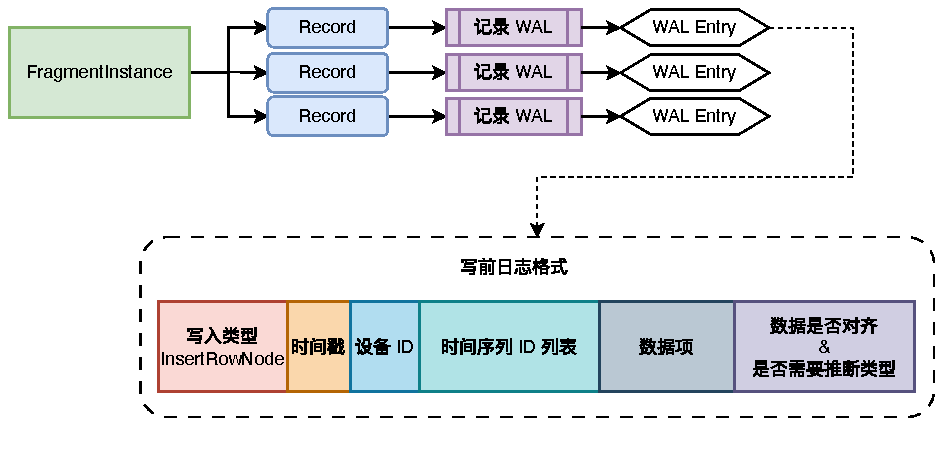
\includegraphics[width=\linewidth]{origin-wal-format.pdf}
  \caption{原有写入日志格式}
  \label{fig:origin-wal-format}
\end{figure}

图 \ref{fig:origin-wal-format} 展示了在原有 IoTDB 的实现中,一个 FragmentInstance 在写入时记录写前日志的流程和格式。对一个 FragmentInstance 中的每一行记录,都需要单独记录一次写前日志,每次都需要重复记录这些记录的时间戳、设备 ID、时间序列 ID 和数值项等,而这其中有相当一部分信息是重复的。这样的设计会导致写前日志的体积过大,对磁盘的写入量也会增加,从而影响写入性能。

\begin{figure}
  \centering
  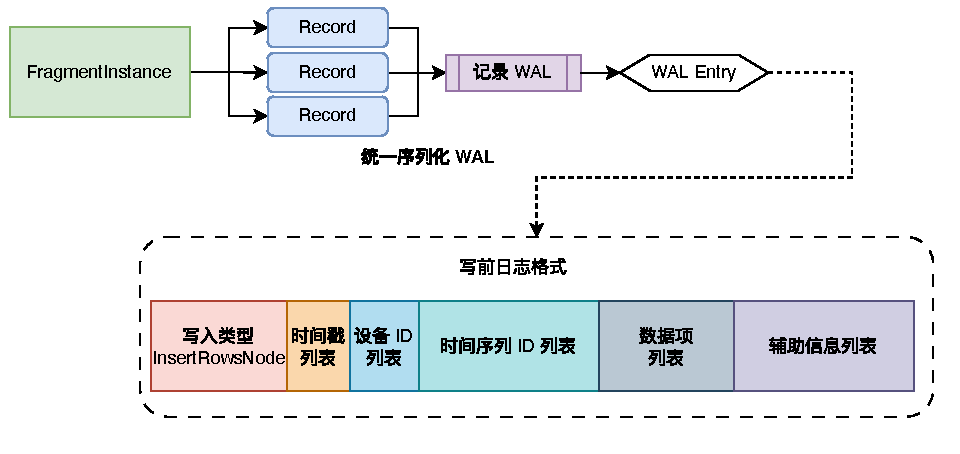
\includegraphics[width=\linewidth]{批量化wal设计.pdf}
  \caption{批量化 WAL 序列化设计}
  \label{fig:batch-wal-design}
\end{figure}

 如果要减小写前日志的体积,我们可以参考第 \ref{sec:chap6} 章的设计,将一个 FragmentInstance 中的所有记录集中在一起序列化,并使用字典压缩、Gorilla 编码等方法针对设备 ID、测点 ID、时间戳等各部分进行针对性的压缩。但是这样会显著增加写入时的 CPU 开销,让每次写入的延迟变高,反而有可能降低写入性能。因此,我们决定结合 \ref{sec:chap7-sec4} 节的工作,先将一个 FragmentInstance 中的所有记录集合在一起,然后将它们的设备 ID、时间序列 ID、时间戳等信息统一序列化到写前日志中,图 \ref{fig:batch-wal-design} 展示了将一个 FragmentInstance 中所有记录一起记录写前日志的设计。这样虽然不能减少写前日志的体积,但是可以将具有具有相似性的数据聚集到一起,提高数据的局部性。而压缩算法通常利用数据的冗余信息来进行压缩,提高数据的局部性可以使得后续对数据进行压缩时的效率变得更高。
\subsubsection{批量化更新监控信息}
 IoTDB 的监控系统负责监控 IoTDB 运行时的各类指标,以便于用户和开发者了解 IoTDB 的状态,并进行运维和调优。
 在 IoTDB 现有的实现中,每写入一个 FragmentInstance 中的一行记录,就需要更新对应的监控信息,包括创建内存表的耗时、写入写前日志的耗时、写入内存表的耗时、更新内存缓存的耗时等。监控系统为这些监控项都维护了对应的直方图,因此每次写入一行记录需要更多这些监控项对应的直方图。从 \ref{sec:chap3-sec3-1} 节中对 \emph{insertRecords} 和 \emph{insertTablets} 的实验中可以看出,\emph{insertRecords} 写入时更新监控信息的开销明显较大。因此,本工作将这些监控信息的更新批量化,每次写入一批数据才更新一次这些监控信息,以减少这些操作对写入性能的影响。

 为了实现这一点,我们修改了更新监控信息的时机和逻辑。每行记录在写入时,仍会记录各个阶段的耗时,但不会将这些耗时立马更新到监控系统里,而是将这些耗时记录在一个本地的数据结构中。这个数据结构只记录这一个写入请求的监控指标,当这个写入请求的每一个 FragmentInstance 都写完了以后,再统一将这些监控指标更新到监控系统中。在这样的设计下,原本执行一次 \emph{insertRecords} 更新监控框架的次数为写入数据的行数,现在则变成了一次,这样就大大减少了更新监控信息对写入性能的影响。

\subsubsection{批量化维护内存缓存}
IoTDB 支持一种名为 Last 查询的查询方式,它可以查询某个时间序列写入数据库的最后一个数据点。为了提高 Last 查询的性能,IoTDB 在内存中维护了一个名为 LastCache 的缓存,其中保存了每个时间序列写入数据库的最后一个数据点。在每次写入时,都需要对这个缓存进行维护。在 IoTDB 的现有实现中,每次写入一行记录都要维护一次这个缓存,这样会导致写入性能下降,从表 \ref{tabular:insert-records-profile-result} 中可以看出,维护内存缓存在 \emph{insertRecords} 写入的性能开销中占有较大的比例。

为了减少维护内存缓存对写入性能的影响,本工作将维护内存缓存的操作批量化,每次写入一个 FragmentInstance 之后才批量化地更新一次缓存。并且,更新缓存之前,先对 FragmentInstance 中的数据进行排序和去重,只更新写入的时间序列的最后一个点。之所以这样设计,是因为 LastCache 的设计比较复杂,反复更新 LastCache 的代价较大,因此我们选择提前处理好数据,以尽可能地减少对 LastCache 的更新。
\subsubsection{批量化写入内存表}
在如今的 \emph{insertRecords} 实现中,写入内存表的操作是行式的,即数据是一行一行地写入到内存表中的。这样的效率并不高,因为每写入一行都要调用许多辅助函数,函数调用的开销无法均摊。此外,这样的写入方式对 CPU 的缓存也并不友好\cite{boncz2005monetdb}。为了提高写入内存表时的效率,本工作将这个过程批量化,在写入之前先对数据进行排序和归类,将写入到同一个内存表的数据聚集到一起,然后一次性地写入到内存表中,以减少函数调用的开销和提高 CPU 缓存的命中率。

\subsection{批量化写入实现}
本工作对上述批量化执行设计进行了实现,下面分别介绍每项工作的实现细节。
\subsubsection{批量化写前日志}
为了将一个 FragmentInstance 中的所有记录一起记录写前日志,我们修改了记录写前日志的位置,将其提前到了内存控制之前。在正式将一个 FragmentInstance 中的所有数据写入到内存表之前,我们会遍历这个 FragmentInstance 中的所有记录,并且使用五个 Buffer 分别记录这些记录的时间戳、设备 ID、时间序列 ID、数据项以及辅助标志数据。当所有记录的内容都被序列化到 Buffer 中后,我们再将这些 Buffer 中的内容依次写入到写前日志中。在这样的实现里,每个 Buffer 中的数据都具有较高的相似性和局部性,即使是使用通用的压缩算法(例如 Snappy、Gzip)也可以获得较好的压缩效果。
\subsubsection{批量化更新监控信息}
\begin{figure}
  \centering
  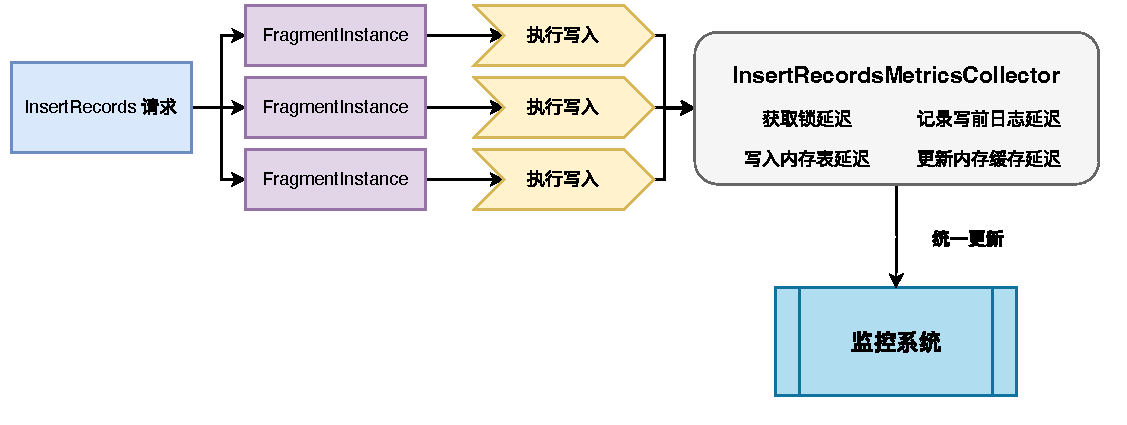
\includegraphics[width=\linewidth]{统一更新监控.pdf}
  \caption{批量化更新监控信息设计}
  \label{fig:batch-update-monitor}
\end{figure}
我们将对监控信息的更新从一行记录更新一次减少为了一个写入请求更新一次,图 \ref{fig:batch-update-monitor} 展示了为了达成这一目的的架构。我们增加了一个名为 InsertRecordsMetricsCollector 的类,这个类的每一个实例都只服务于一个 \emph{insertRecords} 请求。这个类中有若干个 AtomicLong 类型的字段,每个字段分别对应了一个监控指标。每个 FragmentInstance 在执行写入时都会记录自己执行时各个阶段的耗时,并将这些耗时更新到 InsertRecordsMetricsCollector 的对应字段中。当所有 FragmentInstance 都执行完毕以后,主写入线程会将 InsertRecordsMetricsCollector 中的每个字段的值分别更新到监控系统中。

虽然 FragmentInstance 在执行时仍然会多次更新 InsertRecordsMetricsCollector 的字段,但是这些更新都只需要简单的 CAS(Compare And Swap)指令即可完成,而更新监控系统则需要执行对直方图的更新,后者显然更加复杂和耗时。因此,在这样的设计下可以降低写入过程中更新监控信息的开销。
\subsubsection{批量化更新内存缓存}
与批量化更新监控信息类似,我们将更新内存缓存的操作进行了批量化。在更新内存缓存之前,我们会先对 FragmentInstance 中的数据进行排序和去重,保留每个时间序列的最后一个数据点。然后,我们将这些信息一次性更新到内存缓存中,以减少对内存缓存的更新次数。

算法 \ref{alg:batch-update-cache} 展示了批量化更新内存缓存的伪代码。我们使用了一个 Map 来记录每个时间序列的最后一个数据点,最后将这个 Map 中的内容更新到内存缓存中。理论上,LastCache 本身也是一个 Map 结构,但是 LastCache 是一个需要提供全局访问和更新的数据结构,对它的更新会带来同步开销,因此我们选择了先将数据聚集到一个 Map 中,然后再一次性地更新到 LastCache 中,以减少对 LastCache 的更新次数。
\begin{algorithm}
  \caption{批量化更新内存缓存}
  \label{alg:batch-update-cache}
  \small
  \begin{algorithmic}
    \REQUIRE FragmentInstance
    \ENSURE LastCache is updated
    \STATE $n \leftarrow $FragmentInstance.size
    \STATE $lastCache \leftarrow $new HashMap<TimeSeriesId, Pair<Timestamp, Value>>
    \FOR{$i=1$ to $n$}
    \STATE $tsId \leftarrow $FragmentInstance.getTsId($i$)
    \STATE $timestamp \leftarrow $FragmentInstance.getTimestamp($i$)
    \STATE $value \leftarrow $FragmentInstance.getValue($i$)
    \IF{$tsId$ is not in $lastCache$ or $timestamp > lastCache.get(tsId).getKey$}
    \STATE $lastCache.put(tsId, \langle timestamp, value \rangle)$
    \ENDIF
    \ENDFOR
    \STATE Update LastCache with $lastCache$
  \end{algorithmic}
\end{algorithm}
\subsubsection{批量化写入内存表}
在正式写入一个 FragmentInstance 之前,我们将这个 FragmentInstance 中的数据按照写入的内存表进行归类。在 IoTDB 中,一个 DataRegion 会为每一个时间分区维护两个内存表,一个写入顺序数据,一个写入乱序数据。因此,我们只要确定每行记录的时间分区范围以及其顺乱序,就可以确定它们要写到哪个内存表,然后将写入一个内存表的数据聚集到一起,一次性地写入到该内存表中。这样的设计有助于减少写入内存表过程中的固定开销,也有助于提高 CPU 缓存的命中率,进而提高写入性能。
\section{写前日志压缩设计与实现\label{sec:chap7-sec4}}
在 \ref{sec:chap3-sec3-1} 的实验中,我们对比了 \emph{insertRecords} 写入和 \emph{insertTablets} 写入所产生的 WAL 大小和数据文件大小的比值,其中 \emph{insertRecords} 的这一比值为 7:1,是 \emph{insertTablets} 的两倍还多。这也就意味着,在 IoTDB 使用 \emph{insertRecords} 进行写入时,有接近 90\% 的 I/O 资源都用于写前日志的写入,这无疑会影响写入性能。

为了减少 WAL 的大小,节省系统的 I/O 资源,我们对写前日志进行了压缩。下面介绍 WAL 压缩的设计与实现。
\subsection{写前日志压缩设计}
\begin{figure}
  \centering
  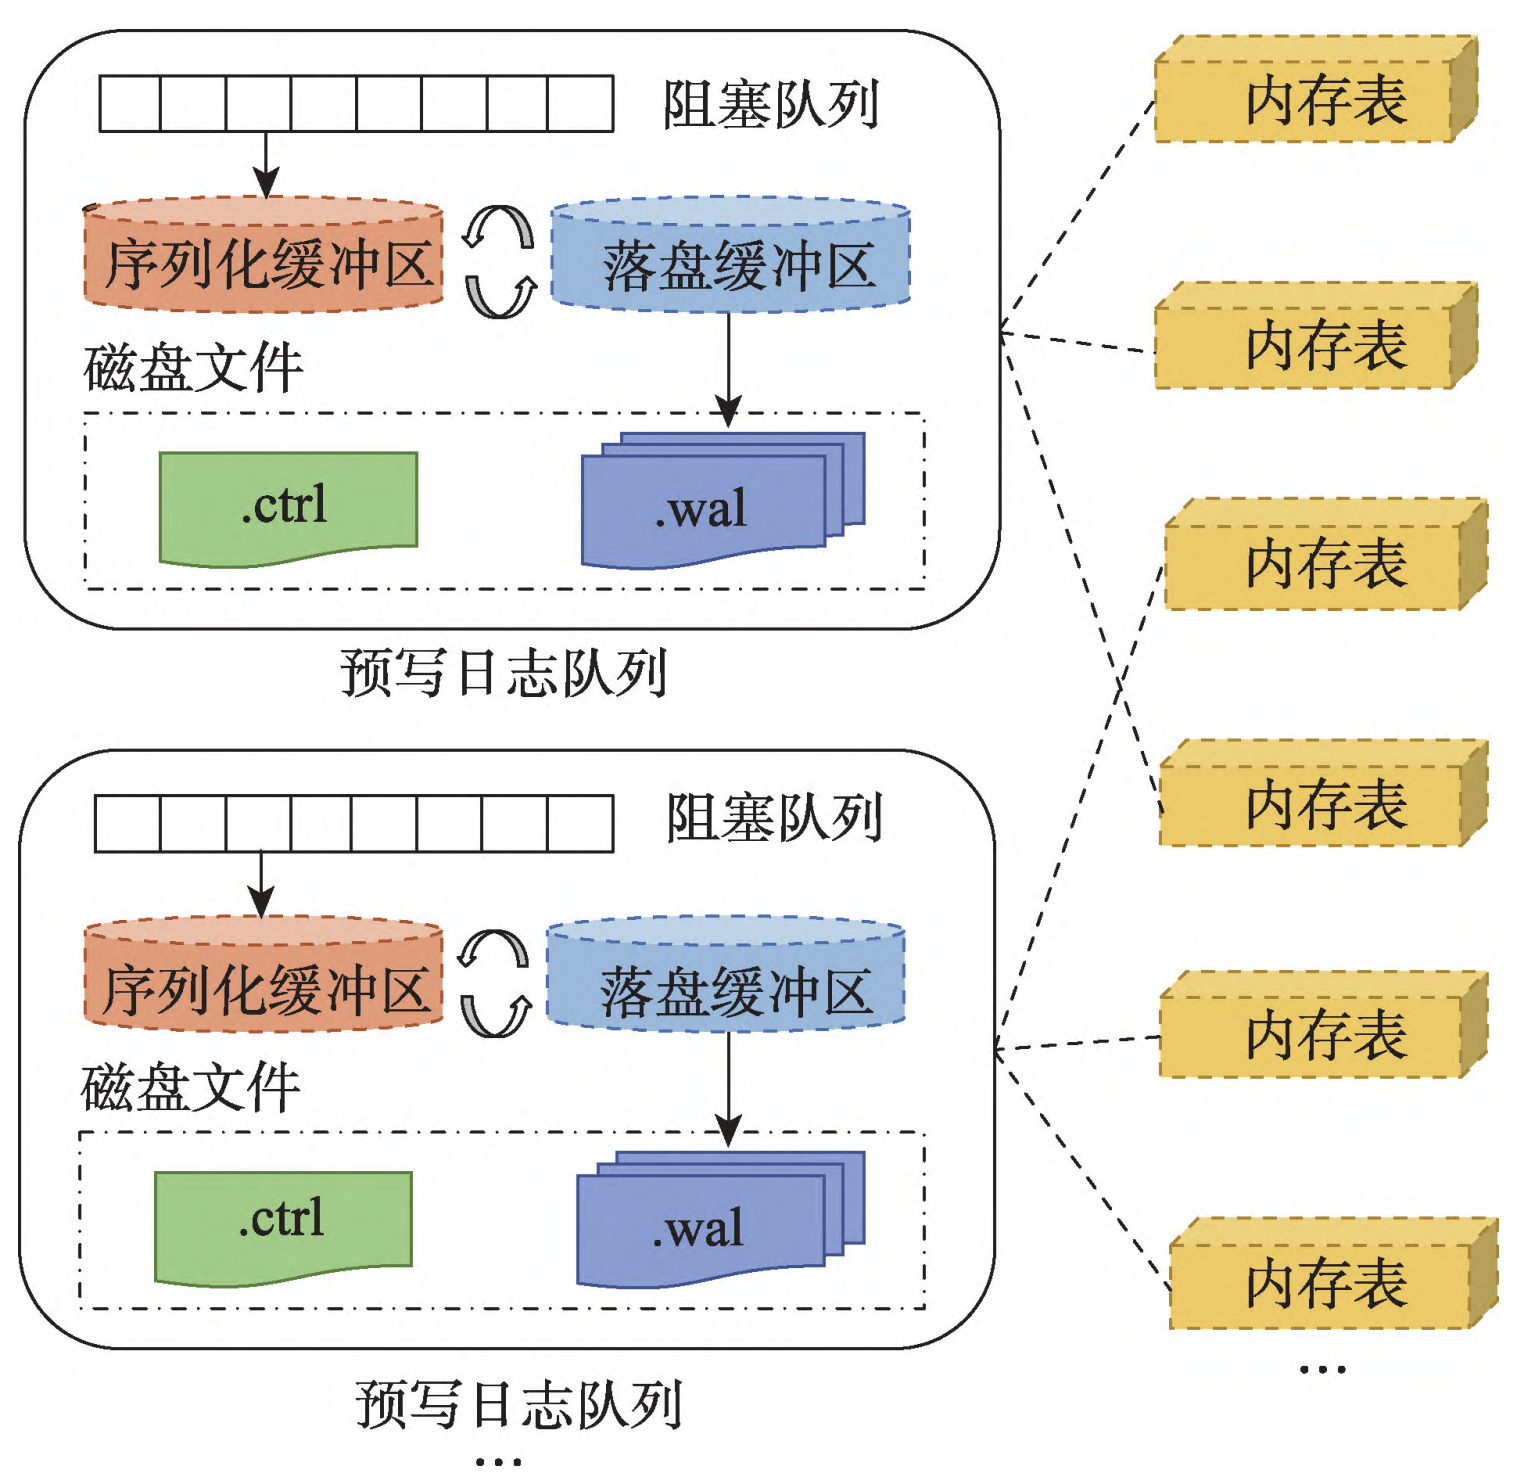
\includegraphics[width=0.7\linewidth]{WAL-structure.png}
  \caption{IoTDB 写前日志结构\cite{朱海铭2023面向内存表的可动态配置预写日志框架}}
  \label{fig:wal-compress-design}
\end{figure}

图 \ref{fig:wal-compress-design} 展示了目前 IoTDB 写前日志系统的结构,多个内存表的写前日志会被写入到同一个 WAL Buffer 中,每个 WAL Buffer 有一个对应的阻塞队列,用于接收异步提交的 WAL 序列化需求。每个 WAL Buffer 都使用了两个内存里的 Buffer 对象来缓存 WAL 序列化后的数据,两个 Buffer 交替使用。当其中一个 Buffer 写满了以后,就会被提交到异步的落盘线程中进行持久化,另一个空 Buffer 则会被用来接收新的 WAL 序列化需求。

对写前日志模块的改动容易牵涉到 IoTDB 中的多个子模块,例如 IoT-Consensus 多副本共识协议、IoTDB 流处理系统都依赖于写前日志中的内容进行数据同步和数据传输。如果按照写前日志项为单位进行压缩,有可能会导致上层应用也需要进行修改,工程量较大。因此,我们的设计需要尽量对上层的应用透明,但是在 I/O 时可以减少写前日志的体积。此外,一个写前日志项序列化出的内容有可能需要多个 WAL Buffer 分别持久化到磁盘上。例如,一个写入中带有 30 MB 的文本,而一个 WAL Buffer 的默认大小是 16 MB,此时该写入请求对应的写前日志就需要通过两个 WAL Buffer 才能完全持久化到磁盘上。在发生这种情况时,针对单一写入日志项的压缩也不易实现。综上,以一个写前日志项为单位的压缩并不是最好的选择,我们选择对整个 WAL Buffer 进行压缩。

对 WAL 的压缩分为两个主要部分:写部分和读部分。在写部分,我们选择在 WAL Buffer 持久化之前对它使用通用压缩算法进行压缩。在读时,需要读取写前日志的模块有存储引擎恢复模块、流处理模块、多副本共识模块等。这些模块对写前日志的读取模式都是先将一块写前日志读入内存,然后解析其中的内容,获取一个个的写前日志项后再继续处理其他上层逻辑。因此,我们在将一个 WAL Buffer 读入内存中时,先将其解压缩,然后将解压缩后的原始 Buffer 进行解析,获取一个个的写前日志项并交由上层应用使用。
\subsection{写前日志压缩实现}
\begin{figure}
  \centering
  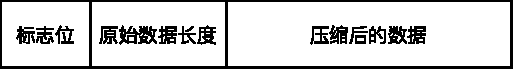
\includegraphics[width=0.7\linewidth]{压缩后WAL的结构.pdf}
  \caption{压缩后的写前日志结构}
  \label{fig:compressed-wal-structure}
\end{figure}
图 \ref{fig:compressed-wal-structure} 展示了压缩后的写前日志结构,我们把这样一个结构称为一个 WAL Segment。在写入时,我们接收到完整的原始 WAL Buffer,然后使用通用压缩算法压缩并记录其原始数据的长度,并且在头部使用一个标记位表示该数据是否被压缩过。之所以需要用标志位,是因为我们把写前日志压缩实现为一个可选的功能。当用户资源不足时,可以不启用写前日志压缩。使用标志位可以保证读取时的兼容性,保证对于压缩和未压缩的写前日志都可以正确解析。

实现压缩的一个关键点是选择合适的压缩算法,IoTDB 目前支持 ZSTD、LZ4、Snappy、LZMA、GZip 等压缩算法。不同压缩算法的压缩率、压缩速度、资源开销各不相同,压缩率越高的往往压缩速度越慢、资源开销越大,反之亦然。经过实验,我们发现 GZip 压缩算法可以取得较好的压缩率和压缩速度,因此我们选择了 GZip 作为 IoTDB 写前日志的压缩算法,具体的实验内容将在第 \ref{sec:chap8} 章中介绍。

在读取时,我们一次读入一个 WAL Segment,然后根据标志位判断是否需要解压缩。如果需要解压缩,就申请一块与原始数据大小相同的内存,然后将压缩后的数据解压缩到这一块内存中,再交由上层应用进行解析。如果不需解压缩,则直接解析 WAL 的数据。这样的设计可以保证对于压缩和未压缩的写前日志都可以正确解析,保证了系统的兼容性。
\section{本章小结}
本章介绍了在存储引擎侧针对 \emph{insertRecords} 写入请求处理进行的若干优化设计,包括多线程并行写入、批量化写入和写前日志压缩。多线程并行写入通过将写入本地 DataRegion 和写入远程 DataRegion 的过程都设计为多线程并行执行,以提高写入性能。批量化写入通过将写前日志、更新监控信息、维护内存索引等操作批量化,减少这些操作对写入性能的影响。写前日志压缩通过对 WAL Buffer 进行压缩,减少写前日志对磁盘的写入量,提高写入性能。